\newpage
\section{Possible Extensions and Improvements}~\label{sec:conclusion}
Our study is not exhaustive. Here are some potential extensions and improvements.
\begin{enumarabic}
  \item Our dataset is not perfect. It is evident in
    ~\cref{tab:count-articles-words} that our data is skewed towards the later years.
    For instance, $2023$ has $3747$ articles, while $2003$ has only $1$ article.
    A potential improvement would be augmenting the dataset with more articles from the earlier years.
    However, this will require some strategy and perhaps access to a corpus of archived articles
    from the prior years, since a naive web crawler like ours will ultimately
    end up visiting a lot of articles from the recent years.
    it is estimated that $90\%$ of the data on the internet was created
    in the last two years~\cite{data-explosion}.

    \begin{figure}[H]
      \centering
      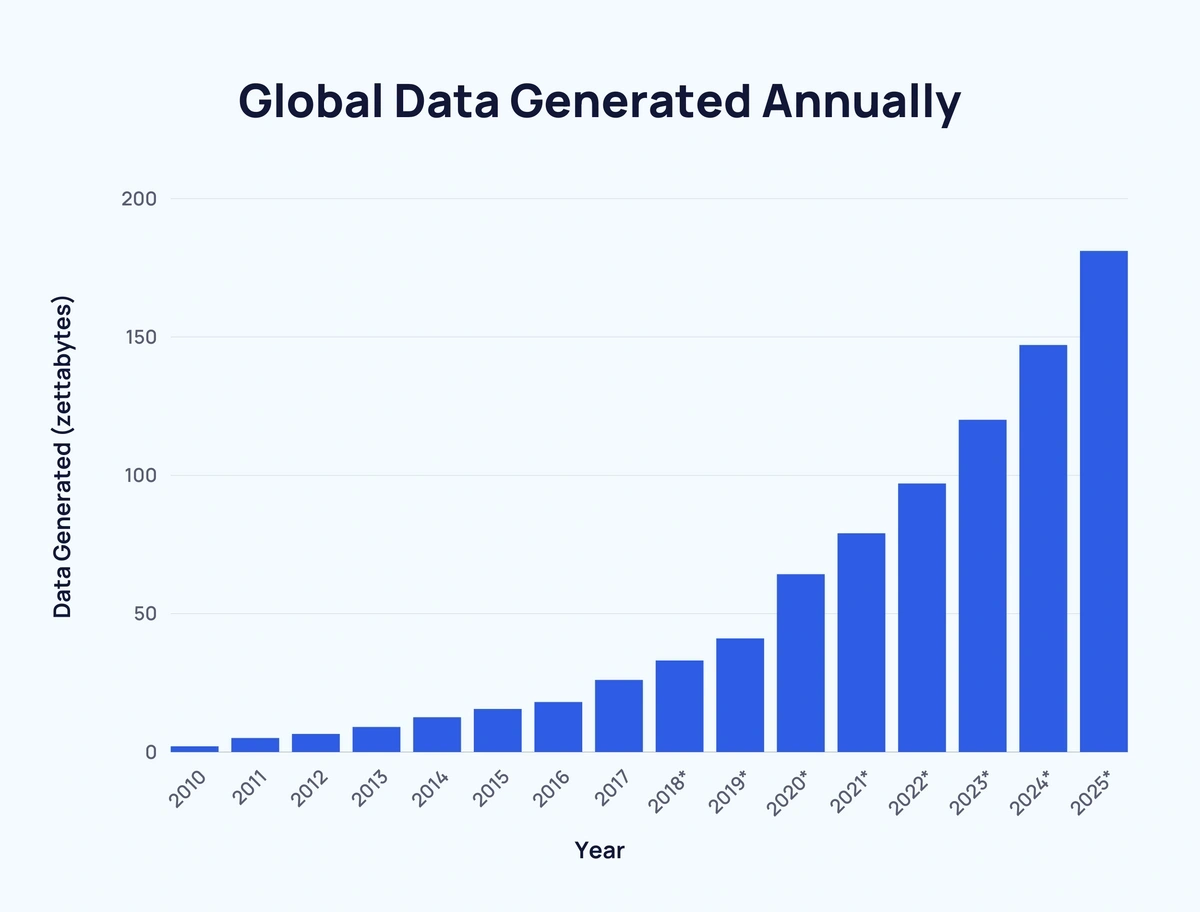
\includegraphics[width=.7\textwidth]{figures/data-explosion.png}
      \caption{Exponential explosion of data on the internet.~\cite{data-explosion}}
    \end{figure}

  \item In cases where we employed topic modeling using LDA,
    it is sometimes noticeable that multiple topics have highly-related top words.
    For examples, see \cref{sub@fig:sentiments-topic-1,sub@fig:sentiments-topic-3}.
    Using a more sophisticated topic modeling technique such as BERTopic~\cite{BERTopic}
    could help group such topics together, and pick out other relevant topics
    from the dataset.
  \item It is also important to note that we are in the middle of a shift
    in how humanity views and talks about AI.
    This means that our study is necessarily an incomplete snapshot of the discourse
    --- in fact, a very significant event (the firing and later rehiring of OpenAI CEO
    Sam Altman~\cite{openai-ceo-event}) happened while we were working on this project,
    and we had to update our dataset to reflect this.
    A future study could look at how the sentiments and trends reflected in our study
    pan out over the next few years.
\end{enumarabic}

\section{Credits}~\label{sec:credits}
We are particularly grateful to Professor Soroush Vosoughi for giving us
a few ideas on how to approach this project,
which kinds of analyses to perform, and how to interpret the results.
